\documentclass{article}
\usepackage{graphicx}
\usepackage{float}

\title{\vspace{-2.5cm}Tabulate Equations of Common Ellipse Parameters}
\author{Dr. Elliot Grafil}
\begin{document}
\maketitle
\section*{Introduction}
This document tabulates the equations needed to deduce any of the six common parameters of an ellipse given two of its parameters. 
\begin{figure}[H]
\begin{center}
\noindent\makebox[\textwidth]{
  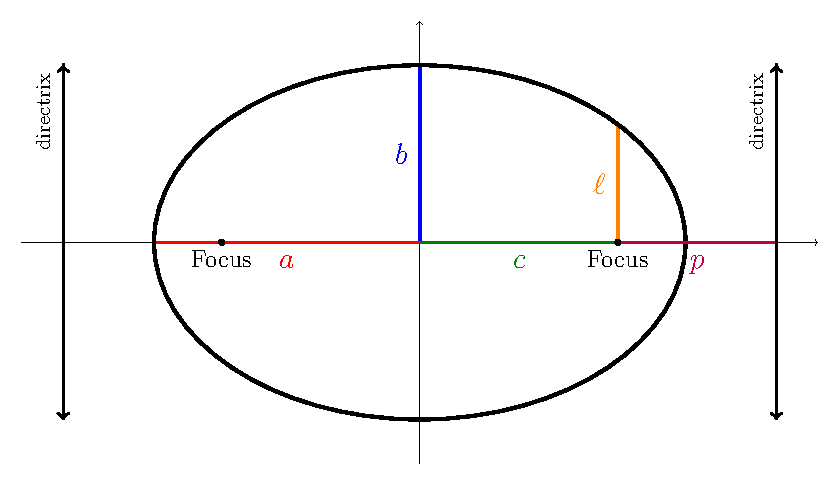
\includegraphics[scale=.75]{./EllipseDiagram/EllipseDiagram.pdf}
  }
  \caption{Common parameters labeled on an example ellipse. Eccentricity, $e$, is not depicted.}
  \label{fig:boat1}
  \end{center}
\end{figure}
\subsection*{\centering{Parameters}}
\begin{description}
\item[$a$] Semi-Major Axis. The length from the center of the ellipse to the farthest point on the curve.
\item[$b$] Semi-Minor Axis. The length from the center of the ellipse to the nearest point on the curve.
\item[$c$] Linear eccentricity. The length from the center of the ellipse to one of its focus.
\item[$e$] Eccentricity. Measurement of deviation from being circular.
\item[$\ell$] Semi-Latus Rectum. The length of a line segment that begins at the focus and makes contact with the ellipse. It is perpendicular to the major axis.
\item[$p$] Focal parameter. The length from one of the two foci to the nearest directrix. 
\end{description}

\subsection*{\centering{Other Useful Relations \& Terminology}}
\begin{description}
\item[Major Axis] Double the length of the semi-major axis ($2a$). The length of the ellipse at its widest point.
\item[Minor Axis] Double the length of the semi-minor axis ($2b$). The length of the ellipse at its thinnest point.
\item[Focal Length] Double the length of the linear eccentricity ($2e$). The length between the ellipse's two foci.
\item[Flattening] A rarer type of measurement for the deviation from being circular. Flattening is given usually in terms of $a$ and $b$ as $f=\frac{a-b}{a}$ or $e$ as $f=1-\sqrt{1-e^2}$. 
\item[Latus Rectum] Double the length of the semi-latus rectum ($2\ell$). The chord that passes through a focus and is perpendicular to the major axis.
\item[Directrix] Focal parameter. The length from one of the two foci to the nearest directrix. 
\end{description}

\subsection*{\centering{Parameters}}
\begin{description}
\item[$a$] Semi-Major Axis.
\item[$b$] Semi-Minor Axis.
\item[$c$] Linear eccentricity.
\item[$e$] Eccentricity. Measurement of deviation from being circular.
\item[$\ell$] Semi-Latus Rectum. The length of a line segment that begins at the focus and makes contact with the ellipse. It is perpendicular to the major axis.
\item[$p$] Focal parameter. The length from one of the two foci to the nearest directrix. 
\end{description}
\newpage

\section*{\centering{Semi-Major Axis}}
\begin{center}
\noindent\makebox[\textwidth]{%
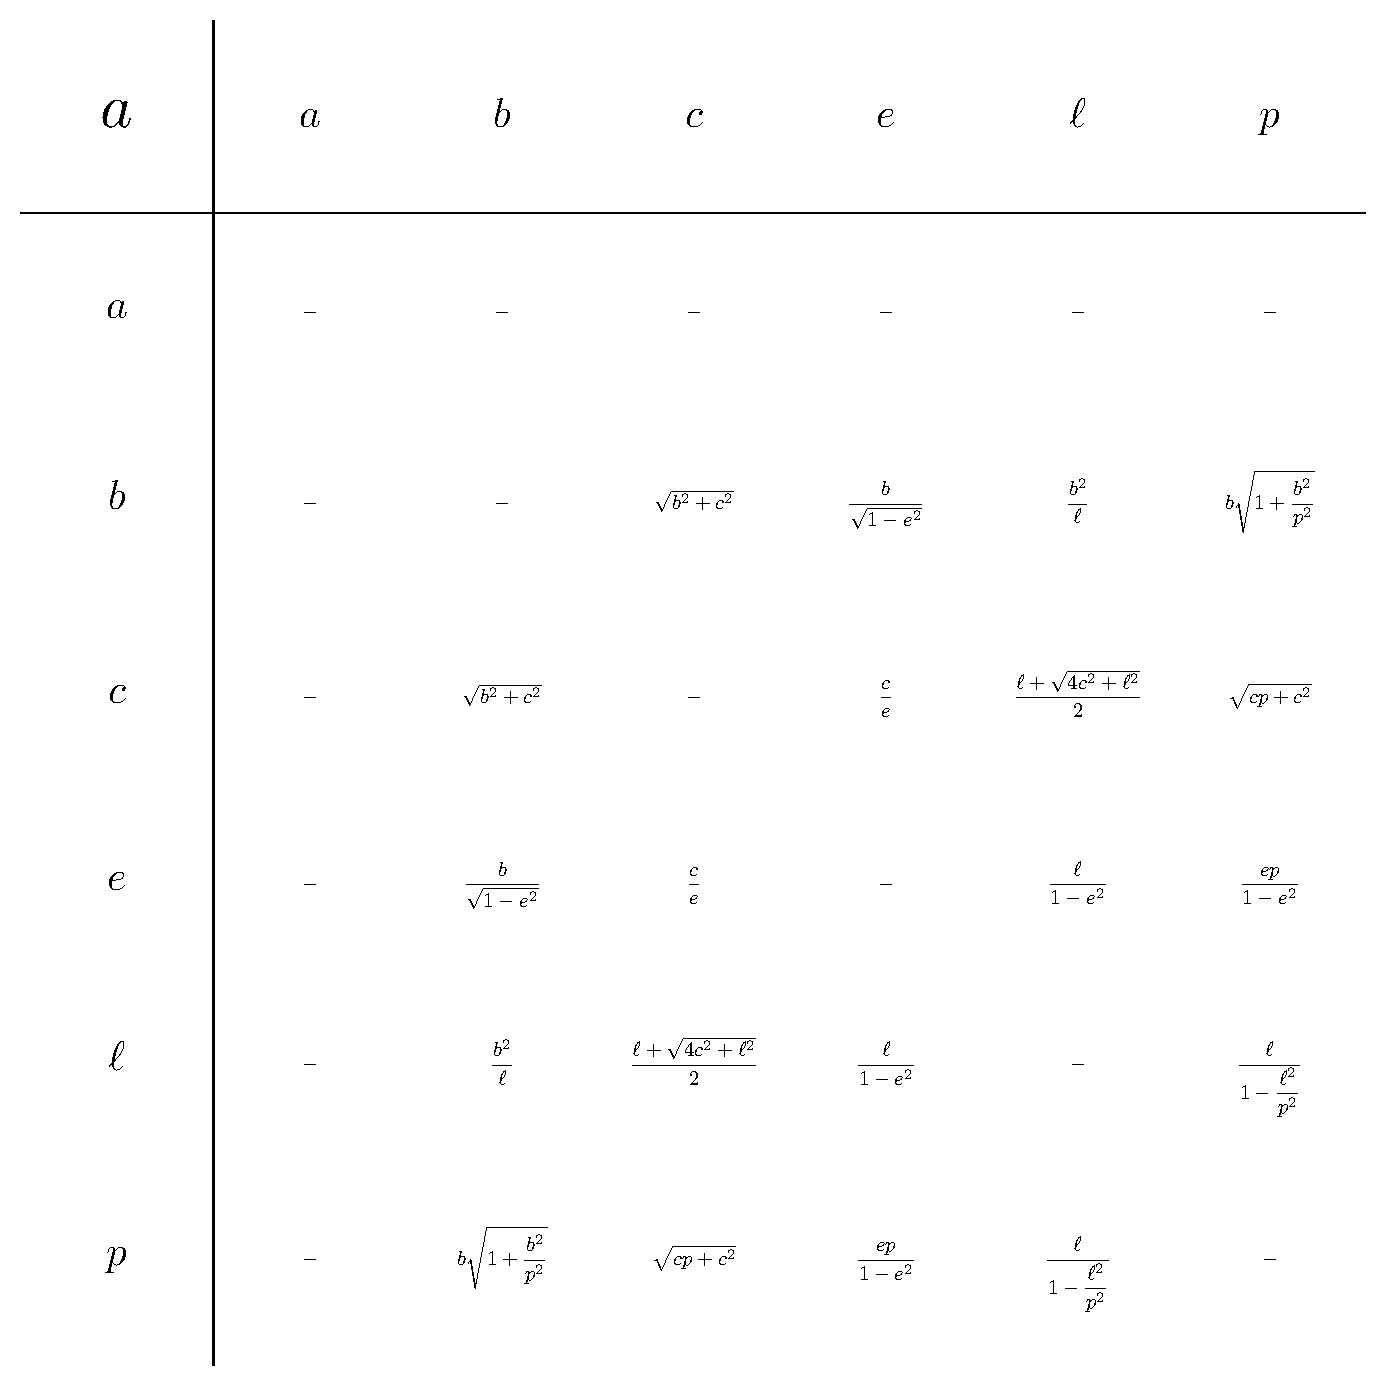
\includegraphics[scale=1]{./AEquation/AEllipseEquations.pdf}
}
\newpage

\section*{\centering{Semi-Minor Axis}}
\noindent\makebox[\textwidth]{%
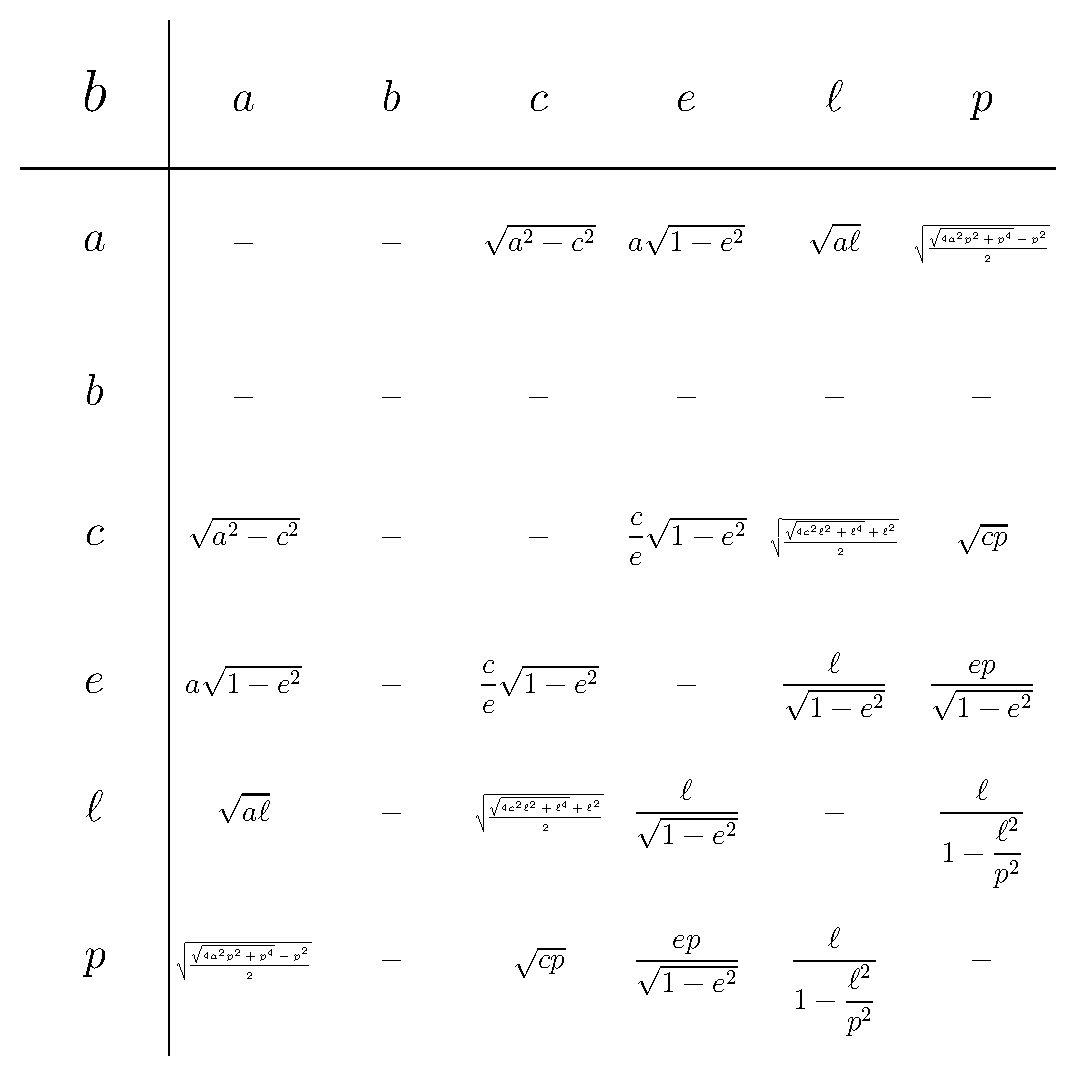
\includegraphics[scale=1]{./BEquation/BEllipseEquations.pdf}
}
\newpage

\section*{\centering{Linear Eccentricity}}
\noindent\makebox[\textwidth]{%
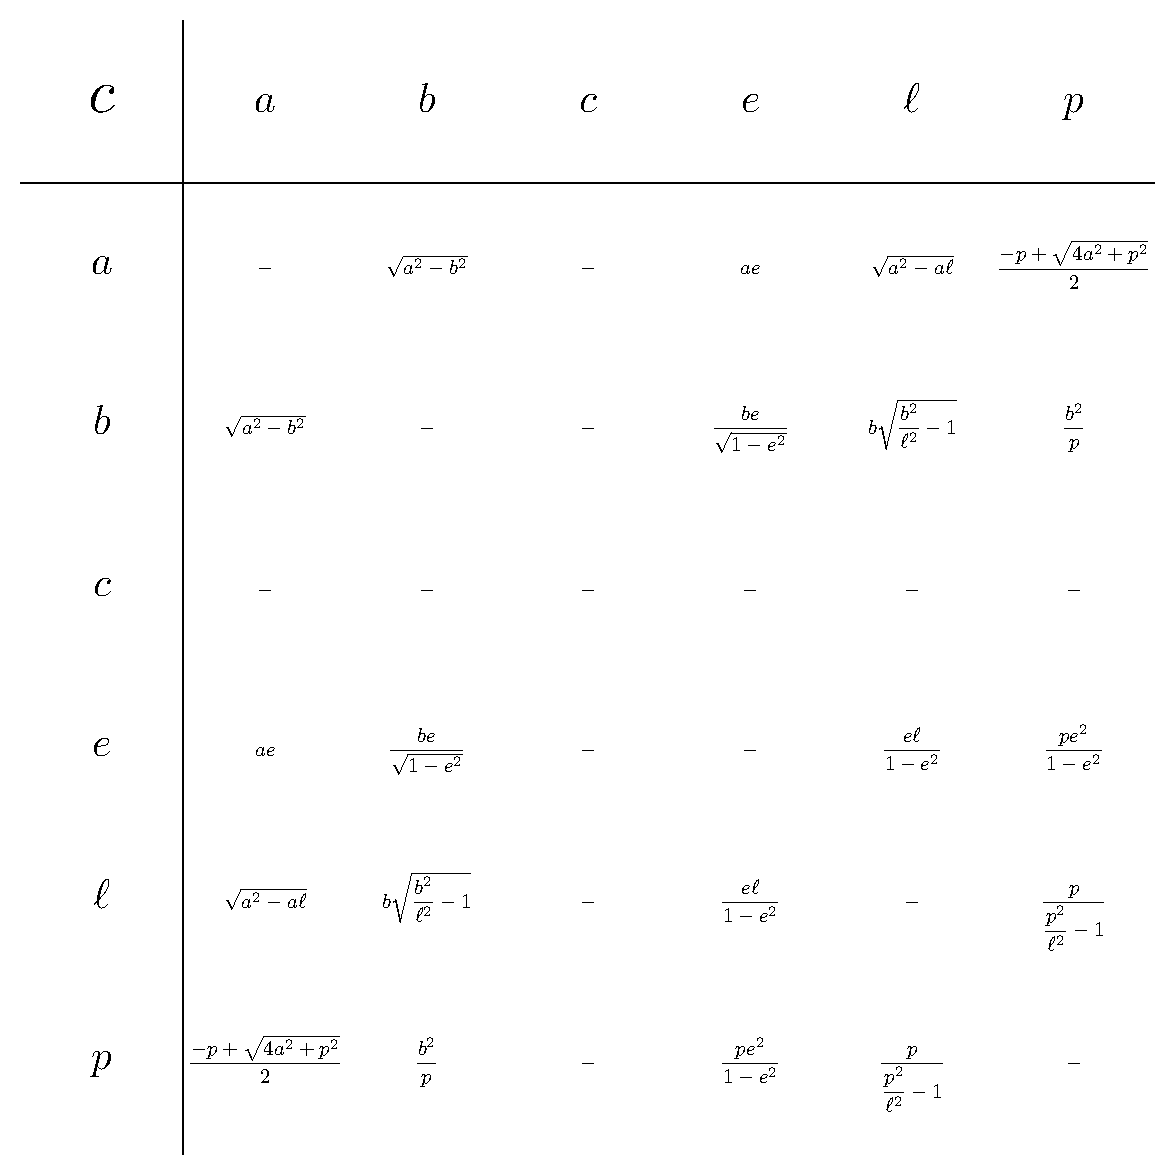
\includegraphics[scale=1]{./CEquation/CEllipseEquations.pdf}
}
\newpage

\section*{\centering{Eccentricity}}
\noindent\makebox[\textwidth]{%
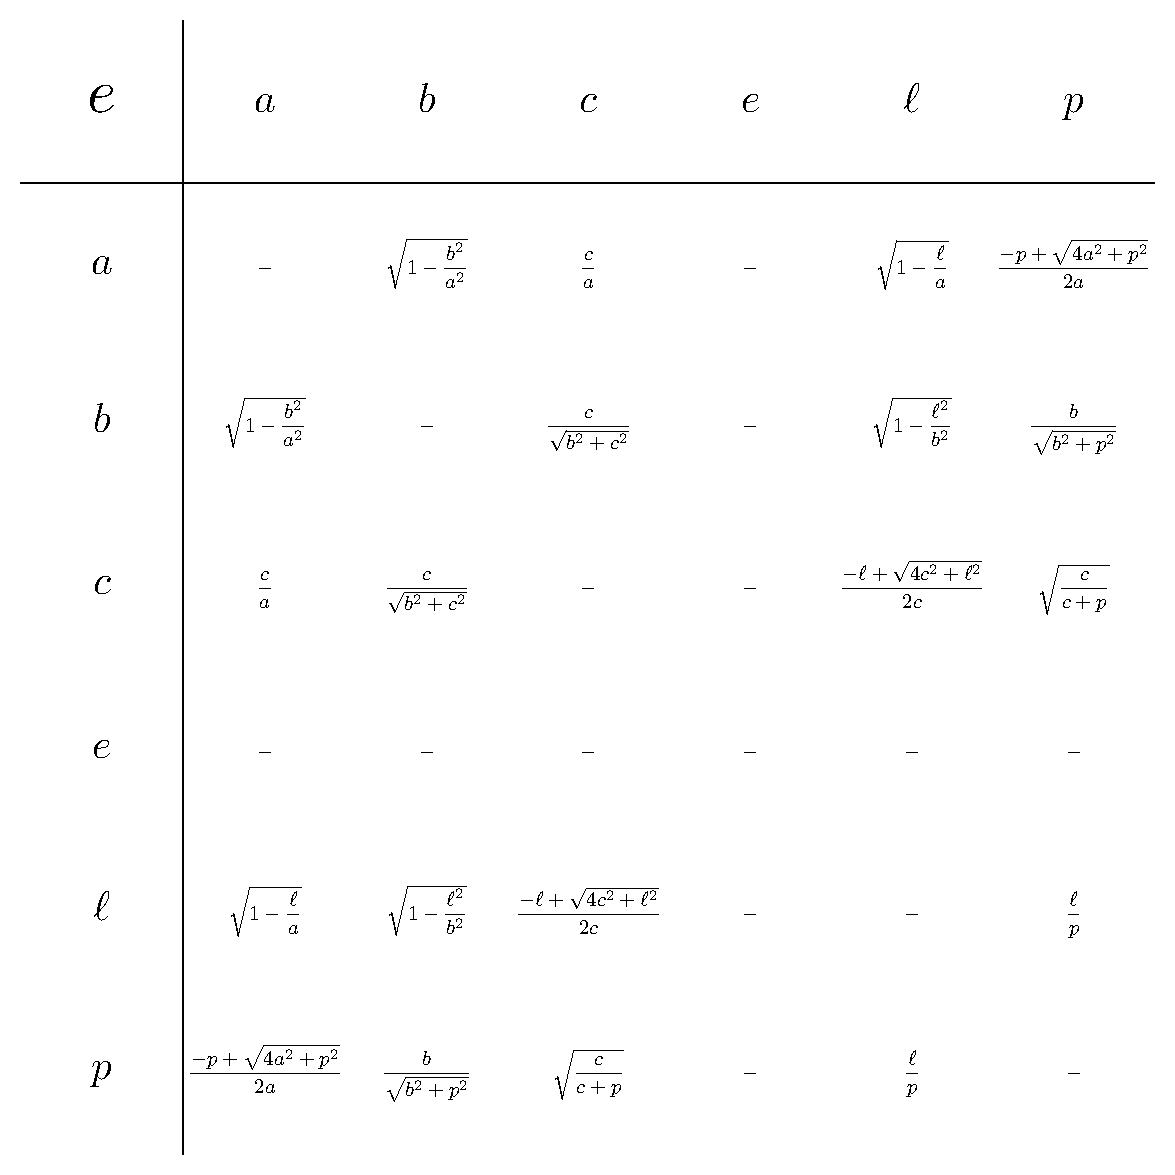
\includegraphics[scale=1]{./EEquation/EEllipseEquations.pdf}
}
\newpage

\section*{\centering{Semi-Latus Rectum}}
\noindent\makebox[\textwidth]{%
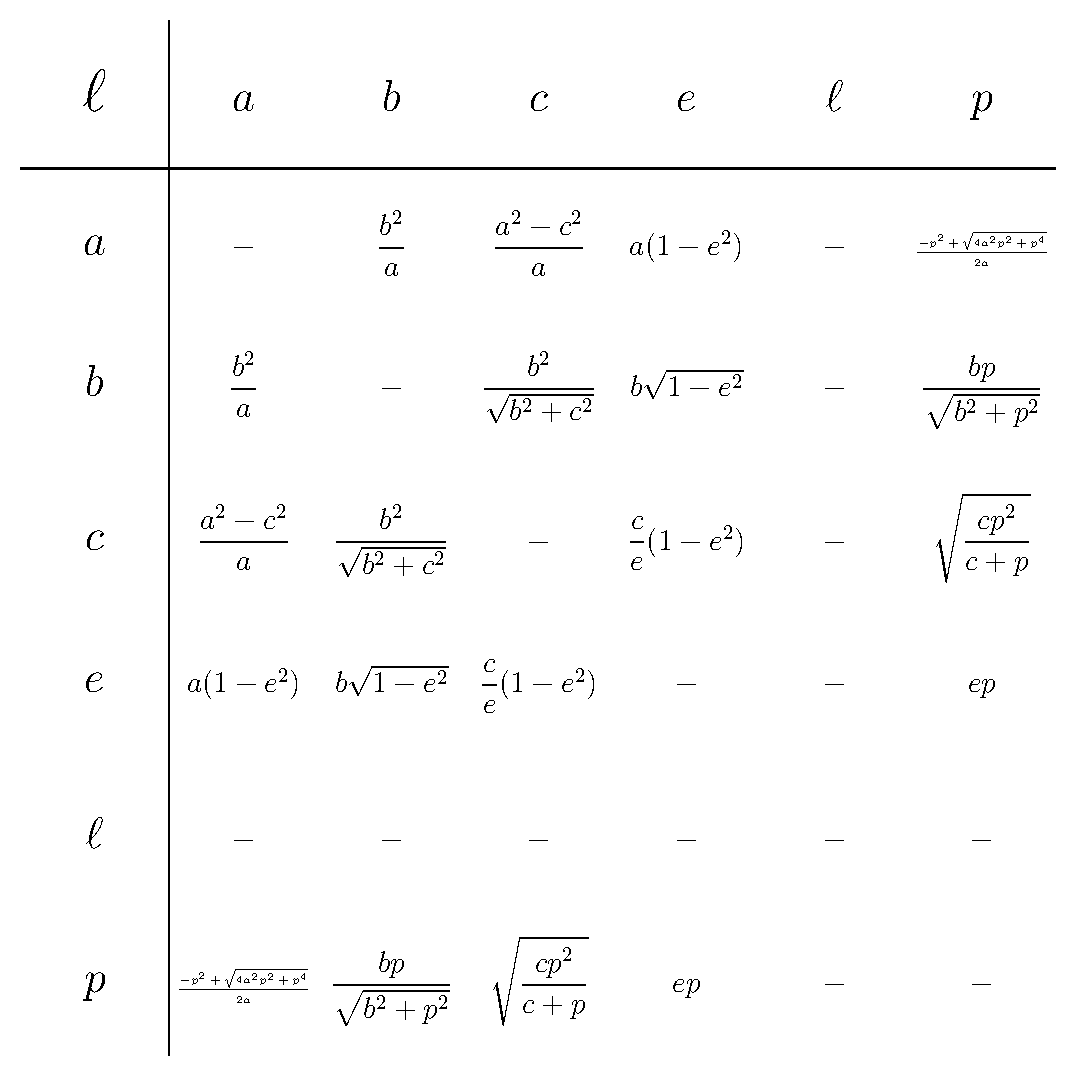
\includegraphics[scale=1]{./LEquation/LEllipseEquations.pdf}
}
\newpage

\section*{\centering{Focal Parameter}}
\noindent\makebox[\textwidth]{%
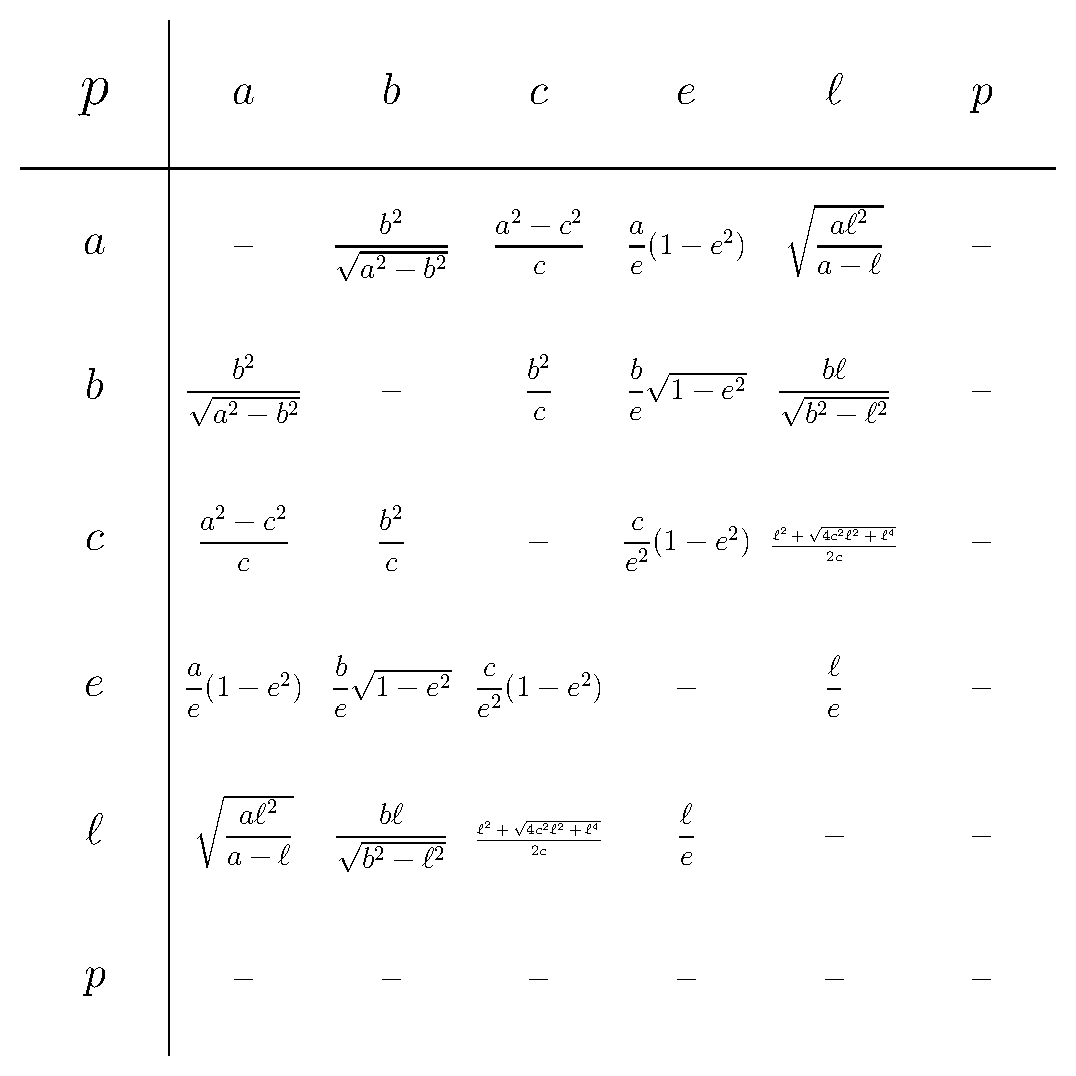
\includegraphics[scale=1]{./PEquation/PEllipseEquations.pdf}
}

\end{center}
\end{document}